
\documentclass[parskip=full,11pt]{scrartcl}
\usepackage[utf8]{inputenc}

\title{Performance Dashboard for Continuous Benchmarking of HPC Libraries}
\author{Chingun Ariunbat, Max Schik, Walter Alexander B�ttcher,\\ Darius Schefer, Jamil Bagga}

% section numbers in margins:
\renewcommand\sectionlinesformat[4]{\makebox[0pt][r]{#3}#4}

% header & footer
\usepackage{scrlayer-scrpage}
\lofoot{\today}
\refoot{\today}
\pagestyle{scrheadings}

\usepackage[sfdefault,light]{roboto}
\usepackage[T1]{fontenc}
\usepackage[english]{babel}
\usepackage[yyyymmdd]{datetime} % must be after babel
\renewcommand{\dateseparator}{-} % ISO8601 date format
\usepackage[colorlinks=true]{hyperref}
\usepackage{amsmath} % for $\text{}$
\usepackage[nameinlink]{cleveref}
\crefname{figure}{Abb}{Abb}
\usepackage[section]{placeins}
\usepackage{xcolor}
\usepackage[nonumberlist]{glossaries}     % provides glossary commands
\usepackage{graphicx}
\hypersetup{
	pdftitle={Pflichtenheft},
	bookmarks=true,
}
\usepackage{csquotes}

\makenoidxglossaries
%
% % Glossareintr�ge
%
\newglossaryentry{developer}
{
	name=Developer,
	plural=Developers,
	description={Person working on the project that is to be benchmarked}
}

\newglossaryentry{Template}
{
	name=template,
	plural=templates,
	description={Configuaration of a visualization}
}

\newacronym{ci}{CI}{Continuous Integration}

\newcommand\urlpart[2]{$\underbrace{\text{\texttt{#1}}}_{\text{#2}}$}

\usepackage{pflichtenheft}

\begin{document}
\maketitle

\section{Introduction}
Glossary acronym example: \\
\acrshort{ci} \\
\acrlong{ci} \\
\acrfull{ci}

\begin{center}
\urlpart{http}{protocol}%
\texttt{://}%
\urlpart{web.io}{host}%
\texttt{/}%
\urlpart{index}{path}%
\texttt{?}%
\urlpart{argument=somevalue}{parameter}%
\texttt{\#}%
\urlpart{theAnchor}{fragment}
\end{center}

more placeholder

\pagebreak
\section{Goals}
% Diese Section sollte kurz und knapp "f�r Manager" sein
% und auf eine Seite passen.

\subsection{Required}

\criterium{heading}{crt:length}

yet more placeholder

\criterium{Schnelle Weiterleitung Kurz- zu Lang-URL}{crt:fast}

\criterium{Authentifizieren mit E-Mail oder Facebook}{crt:login}

\criterium{Rechtlichte Vorgaben werden eingehalten}{crt:tmg}

Der Dienst befolgt alle in Deutschland geltenden Richtlinien,
insbesondere das Telemediengesetz.

\subsection{Optional}

\criteriumOptional{Authentifizieren mit Github}{crt:github}

\criteriumOptional{Seite mit Betreiberinfo}{crt:about}

Der Dienst bietet eine Seite \enquote{�ber Uns},
mit Informationen zum Betreiber.

\subsection{Limitation}

\criteriumNot{Keine Wahl Kurz-URL}{crt:no-choice}

Ein Nutzer hat keine M�glichkeit die Auswahl einer Kurz-URL zu beeinflussen.

\pagebreak
%%%%%%%%%%%%%%
\section{Usage}

Das Produkt soll mit minimalen Administrationskenntnissen zu betreiben sein.

Besucher des Diensts sollen diesen ohne Schulung oder andere Information benutzen k�nnen.

\section{Product Environment}

Das Programm soll als Servlet in einem Apache Tomcat betrieben werden.

Es stehen mindestens 2 AMD64 Kerne mit insgesamt 2GB shared RAM zur Verf�gung.

%%%%%%%%%%%
\section{Functional Requirements}

\functionality{Schnelle Weiterleitung}{fnc:o1}
\fulfills{crt:fast}

Um zu einer Kurz- die Lang-URLs zu finden,
benutzt der Dienst einen $O(1)$ Mechanismus.
Es wird sichergestellt,
dass mit einer zunehmenden Anzahl von Kurz-URLs im System
das Finden nicht l�nger dauert.

\functionality{Login-M�glichkeit auf Homepage}{fnc:login}
\fulfills{crt:login}
\fulfills{crt:github}

Auf der Homepage \texttt{http://atu.rl/} sieht ein Besucher
einen \enquote{Login via Facebook} Knopf.
Weitere Kn�pfe wie \enquote{Login via Github} sind m�glich.
Siehe \cref{fig:homepage}.

\functionality{Auf jeder Seite ist ein Link \enquote{Impressum}}{fnc:impressum-link}
\fulfills{crt:tmg}

Entsprechend Telemediengesetz (TMG) �1
m�ssen gewisse Informationen �ber einen Betreiber jederzeit verf�gbar sein.
Die inzwischen etablierte Vorgehensweise ist auf allen~(!) Seiten
einen Link mit dem Text \enquote{Impressum} anzubieten.
Dieser Link f�r auf eine Seite mit entsprechender Erkl�rung.

\functionality{Auf jeder Seite ist ein Link \enquote{Datenschutz}}{fnc:datenschutz-link}
\fulfills{crt:tmg}

Entsprechend Telemediengesetz (TMG) �13
muss der Betreiber den Nutzer Speicherung und Verarbeitung seiner personenbezogenen Daten unterrichten.
Die inzwischen etablierte Vorgehensweise ist auf allen (!) Seiten
einen Link mit dem Text \enquote{Datenschutz} anzubieten.
Dieser Link f�r auf eine Seite mit entsprechender Erkl�rung.

\functionality{Daten werden persistent gespeichert}{fnc:persistence}

Ein geordneter Neustart des Diensts f�hrt nicht zu Datenverlust.

%%%%%%%%%%%
\section{Nonfunctional Requirements}

\nonFunctionality{Modernes Design}{nfc:design}

Das Design soll modern und seri�s wirken.

\nonFunctionality{Persistenz}{nfc:persistence}

Sollten in Zukunft Erweiterungen oder Updates notwendig werden,
m�ssen die Daten (Kurz-URLs, E-Mailaddressen) erhalten bleiben.

\nonFunctionality{Erweiterbarkeit}{nfc:extensibility}

Das Produkt muss dahingehend erweiterbar sein,
das die Liste der E-Mail-URL Abbildung von authentifizierten Nutzern
abgerufen werden kann.
Wie das genau implementiert wird, ist nicht Teil dieses Projekts.

%%%%%%%%%%%
\section{Tests}

\test{Kurz-URL Erstellen}{tst:create}
\tests{fnc:login}

\teststep{Besucher \enquote{Zoe Washburne} hat einen Browser ge�ffnet.}
{Zoe navigiert auf die Homepage \texttt{http://atu.rl/}.}
{Die Homepage wird angezeigt wie in \cref{fig:homepage}.}

\teststep{Zoe hat einen Facebook-Account.}%
{Zoe dr�ckt den \enquote{Login via Facebook} Knopf.}%
{Zoe wird eingeloggt und auf die Erstellseite wie in \cref{fig:form} weitergeleitet.}

\teststepnostate
{Zoe bef�llt das Feld \enquote{URL} mit \texttt{sehrlangedomain.com/undganzlangeURL.html} und dr�ckt auf \enquote{Kurz-URL erstellen}.}%
{Ihr wird eine Kurz-URL angezeigt wie z.B.\ \texttt{atu.rl/abc}
 wie in \cref{fig:generated}.
 Statt \enquote{abc}, d�rfen beliebige andere Buchstaben und Zahl angezeigt werden, allerdings exakt drei.}

\teststepnostate
{Zoe navigiert auf die eben generierte Kurz-URL, z.B.\ \texttt{http://atu.rl/abc}.}
{Sie wird zu \texttt{sehrlangedomain.com/undganzlang  eURL.html} weitergeleitet.}

\test{Betreiberinfos lesen}{tst:tmg}
\tests{fnc:impressum-link}
\tests{fnc:datenschutz-link}

\teststep{Besucher \enquote{Jayne Cobb} ist auf der Homepage}
{Er folgt dem Link mit dem Text \enquote{Datenschutz}}
{Ein Text mit allen Datenschutzinformationen wird ihm angezeigt.}

\teststepnostate
{Jayne folgt dem Link mit dem Text \enquote{Impressum}}
{Ein Text mit Informationen des Betreibers wird ihm angezeigt.}

%%%%%%%%%%%%%
\pagebreak
\section{Scenarios}

\textbf{Scenario name:} pushAndInspect \\
\textbf{Participating actor instance:} Bopp: \gls{developer}
\begin{itemize}
	\item Bopp pushes his work to a git repository and fires off a benchmarkt test
	\item Bopp opens the web app and selects his last pushed change
	\item Bopp chooses a type of visualization
	\item The app creates the given type of visualization with the benchmark results from the selected change
\end{itemize}

\textbf{Scenario name:} visualizeFromTemplate \\
\textbf{Participating actor instance:} Jeremy: User
\begin{itemize}
	\item Jeremy opens the web app
	\item Jeremy chooses a template for a visualization
	\item Jeremy chooses which commit he wants to visualize
	\item The app creates the given type of visualization with the commit
\end{itemize}

\textbf{Scenario name:} saveTemplate \\
\textbf{Participating actor instance:} Jeremy: User
\begin{itemize}
	\item Jeremy opens the web app
	\item Jeremy configures a visualization
	\item Jeremy saves his visualization as a template for future use
\end{itemize}

\textbf{Scenario name:} inspect \\
\textbf{Participating actor instance:} Jeremy: User
\begin{itemize}
	\item Jeremy wants to see the latest performance benchmarks for the project
	\item Jeremy opens the web app and selects the latest change
	\item Jeremy chooses a benchmark to compare
	\item Jeremy chooses a type of visualization by selecting which value to plot on the x axis and which value on the y axis
	\item The app creates the given type of visualization with the benchmark results from the selected change
\end{itemize}

\textbf{Scenario name:} compareImplementations \\
\textbf{Participating actor instance:} Jeremy: User
\begin{itemize}
	\item Jeremy wants to know which implementation is the fastest
	\item Jeremy opens the web app and selects a benchmark
	\item Jeremy selects commits from different branches containing different implementations
	\item Jeremy chooses a type of visualization by selecting which value to plot on the x axis and which value on the y axis.
	\item The app creates the given type of visualization with the benchmark results from the selected change
\end{itemize}

\textbf{Scenario name:} pushAndCompare \\
\textbf{Participating actor instances:} Bopp: \gls{developer}
\begin{itemize}
	\item Bopp pushes his work to a git repository, and fires off a benchmark test.
	\item Benchmark results are fed into the database.
	\item Bopp opens the webapp and selects his last pushed change>
	\item Bopp selects a previous change that he wants to compare to.
	\item Bopp chooses a type of visualization.
	\item The app creates the given type of visualization with the benchmark results from the selected changes.
\end{itemize}

\textbf{Scenario name:} badPerformance \\
\textbf{Participating actor instances:} Bopp: \gls{developer}
\begin{itemize}
	\item Bopp pushes his work to a git repository, and fires off a benchmark test.
	\item Benchmark results are fed into the database.
	\item Our dashboard-backend realizes that the benchmark data for this change is far worse than usual.
	\item Bopp gets notified that his last pushed change significantly worsened the performance and the related details about that.
\end{itemize}

\textbf{Scenario name:} impossiblePerformance \\
\textbf{Participating actor instances:} Bopp: \gls{developer}
\begin{itemize}
	\item Bopp pushes his work to a git repository, and fires off a benchmark test.
	\item Benchmark results are fed into the database.
	\item Our dashboard-backend realizes that the benchmark data for this change is theoretically impossible.
	\item Bopp gets notified that his last pushed change has improved the performance above the theoretical maxiumum and the related details about that.
\end{itemize}

\textbf{Scenario name:} authentification \\
\textbf{Participating actor instance:} Jeremy: User
\begin{itemize}
	\item Jeremy opens the webapp.
	\item Jeremy gets prompted for a authentification.
	\item Jeremy logs in over Github/Gitlab/other services.
\end{itemize}

\textbf{Scenario name:} shareVisualization \\
\textbf{Participating actor instance:} Jeremy: User
\begin{itemize}
	\item Jeremy found an interesting visualization for something.
	\item Jeremy clicks a *share* button next to the visualization.
	\item Jeremy gets a link he can share with others that redirects them to the exact same visualization.
\end{itemize}

\textbf{Scenario name:} visualizeCommitWithoutBenchmark\\
\textbf{Participating actor instance:} Jeremy: User
\begin{itemize}
	\item Jeremy opens the webapp and wants to visualize benchmarkdata for a specific commit. This commit has no benchmark data attached to it, only the commit before and the commit after.
	\item Jeremy can't click on the commit because it is greyed out.
\end{itemize}

\textbf{Scenario name:} takeVisualizationFromHistory\\
\textbf{Participating actor instance:} Jeremy: User
\begin{itemize}
	\item Jeremy opens the webapp and visualizes something. He then visualizes something else. His previous visualizations are stored in a list somewhere.
	\item Jeremy decides to take another look at a previous visualization.
	\item Jeremy picks his previous visualization and gets the previous visualization.
\end{itemize}


\appendix

\section{Seitenentw�rfe}

% made via https://gomockingbird.com/projects/mnf0cwf/4gXVnC

\begin{figure}[hb]
\fbox{
\includegraphics[width=\textwidth]{image/login.png}}
\caption{\label{fig:homepage}
Homepage mit Login-Funktion
}
\end{figure}

\begin{figure}[hb]
\fbox{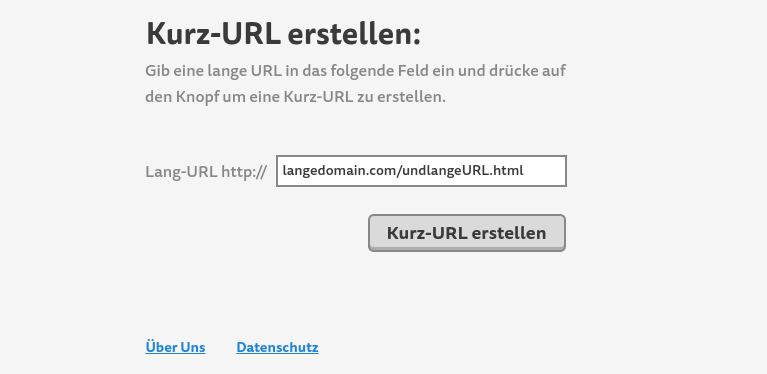
\includegraphics[width=\textwidth]{image/form.png}}
\caption{\label{fig:form}
Formular zur Generierung einer Kurz-URL.
Getestet beispielsweise in \testlink{tst:create}.
}
\end{figure}

\begin{figure}[hb]
\fbox{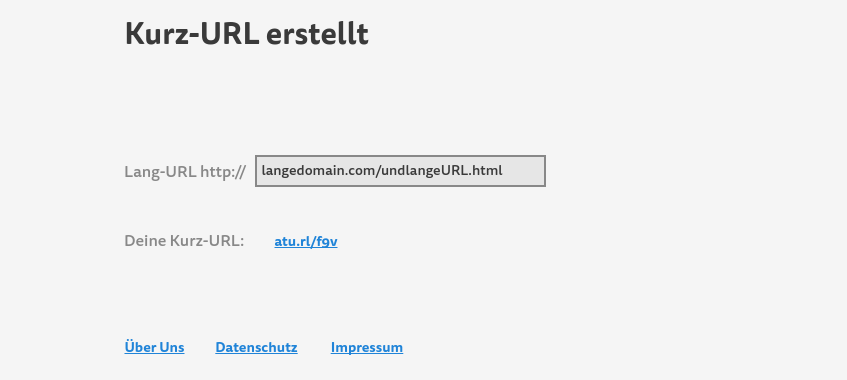
\includegraphics[width=\textwidth]{image/generated.png}}
\caption{\label{fig:generated}
Anzeige der generierten Kurz-URL.
Das Textfeld mit der Lang-URL kann nicht ge�ndert werden.
}
\end{figure}

\printnoidxglossaries

\end{document}
